$xyz$ 空間において次のような3つの互いに合同な長方形 $L_1, L_2, L_3$ を考える。
\begin{itemize}
  \item $L_1$ は $xy$ 平面に含まれ、$P_1(a, b, 0)$, $Q_1(-a, b, 0)$, $R_1(-a, -b, 0)$, $S_1(a, -b, 0)$ を頂点とする。
  \item $L_2$ は $yz$ 平面に含まれ、$P_2(0, a, b)$, $Q_2(0, -a, b)$, $R_2(0, -a, -b)$, $S_2(0, a, -b)$ を頂点とする。
  \item $L_3$ は $zx$ 平面に含まれ、$P_3(b, 0, a)$, $Q_3(b, 0, -a)$, $R_3(-b, 0, -a)$, $S_3(-b, 0, a)$ を頂点とする。
\end{itemize}
ここで $a > b > 0$ とする。このとき次の間に答えよ。

\begin{enumerate}
  \item $\triangle P_1 P_2 P_3$ の面積、および $\triangle P_1 P_2 P_3$ と原点 $O$ との距離を求めよ。
  \item 四面体 $O P_1 P_2 P_3$ および四面体 $O P_1 P_2 S_2$ の体積をそれぞれ求めよ。
  \item $L_1, L_2, L_3$ の12頂点から3点を選び三角形をつくる。このとき $\triangle P_1 P_2 P_3$ または $\triangle P_1 P_2 S_2$ と合同な三角形が20個えられる。これらの三角形で囲まれる立体を $D$ とする。 $0 < \theta < \frac{\pi}{4}$ なる $\theta$ に対して
        \[
          a = \cos \theta, \quad b = \sin \theta
        \]
        とおくとき $D$ の体積 $V$ を $t = \tan \theta$ の関数 $V(t)$ として表せ。
  \item $0 < t < 1$ において $V(t)$ は最大値をとることを示し、そのときの $t$ の値を求めよ。
\end{enumerate}

\begin{figure}[H]
  \centering
  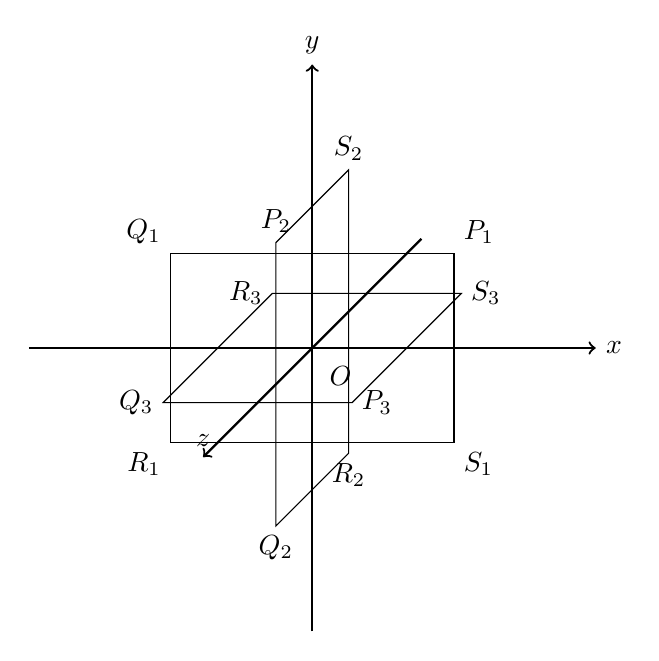
\begin{tikzpicture}[scale=1.2]
    \draw[thick, ->] (-3,0) -- (3,0) node[right] {$x$};
    \draw[thick, ->] (0,-3) -- (0,3) node[above] {$y$};
    \draw[thick, ->] (0,0,-3) -- (0,0,3) node[above] {$z$};
    \node at (0.3,-0.3,0) {$O$};

    \draw (1.5,1,0) node[above right] {$P_1$} -- (-1.5,1,0) node[above left] {$Q_1$} -- (-1.5,-1,0) node[below left] {$R_1$} -- (1.5,-1,0) node[below right] {$S_1$} -- cycle;
    \draw (0,1.5,1) node[above] {$P_2$} -- (0,-1.5,1) node[below] {$Q_2$} -- (0,-1.5,-1) node[below] {$R_2$} -- (0,1.5,-1) node[above] {$S_2$} -- cycle;
    \draw (1,0,1.5) node[right] {$P_3$} -- (-1,0,1.5) node[left] {$Q_3$} -- (-1,0,-1.5) node[left] {$R_3$} -- (1,0,-1.5) node[right] {$S_3$} -- cycle;
  \end{tikzpicture}
\end{figure}
